\section{Carrier, compensator and sectors}
\label{sec:A-carrier}

This section collects the mathematics on which everything else rests. All statements in it are
\Established, with proofs that fit on a few lines. The physical names attached to the objects
(matter, light, tachyon) are a \Reading{} and are marked as such.

\subsection{The biquaternion kernel}
\label{sec:A-kernel}

\begin{definition}[Biquaternion kernel; \cite{QSC}, \texttt{def:biquaternion}]
\label{def:A-kernel}
Let $e_1,e_2$ be imaginary quaternion units and $e_3=e_1e_2$. A kernel is a biquaternion
\begin{equation}
q=it\,\mathbf 1+z_1e_1+z_2e_2+z_3e_3\in\mathbb C\otimes_{\mathbb R}\mathbb H,
\qquad t\in\mathbb R,\quad z=(z_1,z_2,z_3)\in\mathbb C^3 .
\label{eq:A-kernel}
\end{equation}
The three complex coefficients $z_k$ are the three \emph{complex kernels} $K_1,K_2,K_3$ of the
construction. The complex unit $i$ commutes with the quaternion units.
\end{definition}

The original definition equipped $q$ with the Hermitian norm $-t^2+\sum_k|z_k|^2$ and read it as a
Minkowski metric. Round v4.8.0-r06 corrected this: as a real quadratic form in the seven real
variables $(t,\operatorname{Re}z_k,\operatorname{Im}z_k)$ it has signature $(1,6)$, and conjugation by
real unit quaternions only rotates $\operatorname{Re}z$ and $\operatorname{Im}z$, each by the same spatial rotation; it
contains no boost. The invariant that the algebra provides is a different one.

\begin{proposition}[Natural norm; v4.8.0-r06.1]
\label{prop:A-norm}
Let $\bar q=it\,\mathbf 1-z_1e_1-z_2e_2-z_3e_3$ be quaternion conjugation without complex
conjugation. Then
\begin{equation}
N(q):=q\bar q=-t^2+s(z),\qquad s(z)=z_1^2+z_2^2+z_3^2,
\label{eq:A-norm}
\end{equation}
and $N(pq)=N(p)N(q)$.
\end{proposition}

\begin{proof}
Write $q=it+\mathbf z$ with $\mathbf z=\sum_kz_ke_k$. The coefficients commute with the units, so
$q\bar q=(it)^2+it(-\mathbf z)+\mathbf z(it)-\mathbf z^2=-t^2-\mathbf z^2$. In
$\mathbf z^2=\sum_{j,k}z_jz_ke_je_k$ the mixed terms cancel because $e_je_k=-e_ke_j$ for $j\neq k$, and
$e_k^2=-1$ gives $\mathbf z^2=-s(z)$. Multiplicativity follows from $\overline{pq}=\bar q\,\bar p$ and
the fact that $N(q)$ is a scalar.
\end{proof}

The working reading of the kernel since v4.8.0-r06 (``Reading~B'', an author decision) takes $z$ as
the carrier of the Lorentz group: conjugation $q\mapsto uqu^{-1}$ with $u\in\mathbb C\otimes\mathbb H$,
$N(u)=1$, fixes the scalar part and acts on $z$ by $SO(3,\mathbb C)$, and
$SO(3,\mathbb C)\cong PSL(2,\mathbb C)\cong SO^+(1,3)$. In this reading $z$ is the
Riemann--Silberstein vector of an electromagnetic field \cite{A-BBB2013},
\begin{equation}
z=\mathbf E+i\mathbf B,\qquad
s=z\cdot z=|\mathbf E|^2-|\mathbf B|^2+2i\,\mathbf E\cdot\mathbf B ,
\label{eq:A-s}
\end{equation}
so that $s$ collects the two Lorentz invariants of the field (units with $c=1$). The scalar $t$ is
an invariant parameter, not the time coordinate of a four-vector. Its role is \Open; on the null set
$N(q)=0$ it would be tied to $s$ by $s=t^2$ (v4.8.0-r07), a candidate that has not been adopted.

The motivating ``triole'' of three kernels with equal moduli and phases $120^\circ$ apart also
finds an exact place here.

\begin{proposition}[Triole; v4.8.0-r06.2]
\label{prop:A-triole}
For $z\in\mathbb C^3$, $\;z_1+z_2+z_3=0$ and $s(z)=0$ hold together if and only if
$z=c\,(1,\omega,\omega^2)$ up to order, with $\omega=e^{2\pi i/3}$ and $c\in\mathbb C$.
\end{proposition}

\begin{proof}
With the elementary symmetric functions $e_1,e_2,e_3$ of the $z_k$ one has $s=e_1^2-2e_2$. So
$e_1=s=0$ gives $e_2=0$, and the $z_k$ are the roots of $\lambda^3-e_3$, the three cube roots of $e_3$.
Conversely $1+\omega+\omega^2=0$ and $1+\omega^2+\omega^4=0$.
\end{proof}

The triole is therefore a centred null configuration. Centring alone does not force $s=0$:
$z=(1,-1,0)$ is centred and has $s=2$.

\subsection{The compensator}
\label{sec:A-compensator}

The second ingredient is a projector built from an involution. Since round v4.8.0-r04 it is defined
and proved on its own, without reference to that earlier manuscript.

\begin{definition}[Heisenberg compensator; v4.8.0-r04.1]
\label{def:A-compensator}
Let $V$ be a real or complex Hilbert space and $J:V\to V$ a linear involution that is self-adjoint,
$J^2=1$, $J^*=J$ (equivalently, an orthogonal or unitary involution). The \emph{compensator} and its
partner are
\begin{equation}
C=\tfrac12(1+J),\qquad A=\tfrac12(1-J).
\label{eq:A-compensator}
\end{equation}
\end{definition}

\begin{proposition}[Compensator as orthogonal projection; v4.8.0-r04.2]
\label{prop:A-compensator}
$C$ and $A$ are complementary orthogonal projections: $C^2=C=C^*$, $A^2=A=A^*$, $CA=AC=0$, $C+A=1$.
Their ranges are $\operatorname{ran}C=\ker(J-1)$ and $\operatorname{ran}A=\ker(J+1)$, and
$C(Jf)=Cf$, $A(Jf)=-Af$ for all $f$.
\end{proposition}

\begin{proof}
$C^2=\tfrac14(1+2J+J^2)=\tfrac12(1+J)=C$, and $C^*=C$ because $J^*=J$; the same computation with $-J$
gives $A$. $CA=AC=\tfrac14(1-J^2)=0$ and $C+A=1$. From $JC=\tfrac12(J+1)=C$, $J$ acts as $1$ on
$\operatorname{ran}C$; conversely $Jf=f$ gives $Cf=f$. Hence $\operatorname{ran}C=\ker(J-1)$, and likewise
$JA=-A$ gives $\operatorname{ran}A=\ker(J+1)$. Finally $CJ=C$ and $AJ=-A$.
\end{proof}

So $C$ keeps the part of a state that $J$ leaves fixed and removes the part that $J$ reverses, and the
two parts are orthogonal. Nothing beyond $J^2=1$ and $J^*=J$ is used. The main-text statement
of \texttt{prop:compensator}, that $C$ ``takes matter and its tachyon image and produces the photon'',
does not follow from this; Section~\ref{sec:A-field-example} shows why.

\paragraph{The field instance.}
On the field $z=\mathbf E+i\mathbf B$ the involution used by the Companion is the exchange of
electric and magnetic field,
\begin{equation}
J_Bz=i\bar z,\qquad J_B(\mathbf E+i\mathbf B)=\mathbf B+i\mathbf E .
\label{eq:A-JB}
\end{equation}
On $\mathbb C^3$ it is antilinear, but on the real space of pairs $(\mathbf E,\mathbf B)\cong\mathbb R^6$
it is linear, orthogonal and symmetric, so Proposition~\ref{prop:A-compensator} applies over $\mathbb R$.
Writing the field as the real $3\times2$ matrix $F=[\,\mathbf E\mid\mathbf B\,]$, $J_B$ acts as
$F\mapsto F\sigma_x$ and the compensator as $F\mapsto FC_{\rm HC}$ with
$C_{\rm HC}=\tfrac12(1+\sigma_x)$ (\rndold{r04}). From \eqref{eq:A-compensator},
\begin{equation}
Cz=(1+i)\,\frac{\mathbf E+\mathbf B}{2},\qquad Az=(1-i)\,\frac{\mathbf E-\mathbf B}{2}.
\label{eq:A-Cz}
\end{equation}
In the kept part both field vectors are equal to $(\mathbf E+\mathbf B)/2$; in the removed part they
are opposite.

\subsection{Sectors by the sign of \texorpdfstring{$s$}{s}}
\label{sec:A-sectors}

The invariant $s$ sorts the field configurations. The following proposition is the exact content of
the sector rule.

\begin{proposition}[Orbits and sectors; v4.8.0-r06.3, r06.4, r07.1, r07.2]
\label{prop:A-orbits}
Let $SO(3,\mathbb C)$ act on $\mathbb C^3$ and let $U(1)_{\rm dual}$ act by $z\mapsto e^{i\alpha}z$.
\begin{enumerate}
\item[(a)] The $SO(3,\mathbb C)$-orbits are the level sets $\{s=c\}$ for $c\neq0$, the punctured null
  cone $\{s=0\}\setminus\{0\}$, and $\{0\}$.
\item[(b)] $s(e^{i\alpha}z)=e^{2i\alpha}s(z)$. In particular the quarter turn $z\mapsto iz$ maps
  $s\mapsto-s$ and preserves the null cone.
\item[(c)] Every $z$ with $s(z)\neq0$ is $z=e^{i\alpha}z_m$ with $s(z_m)=|s(z)|>0$; the angle
  $\alpha=\tfrac12\arg s(z)$ is fixed modulo $\pi$. The configuration has $s>0$ exactly for
  $\alpha\equiv0$ and $s<0$ exactly for $\alpha\equiv\pi/2\pmod\pi$.
\item[(d)] The orbits of $SO(3,\mathbb C)\times U(1)_{\rm dual}$ on $\mathbb C^3\setminus\{0\}$ are the
  shells $\{|s|=r\}$, $r>0$, and the punctured null cone. The null cone is the only orbit fixed by the
  whole duality circle.
\end{enumerate}
\end{proposition}

\begin{proof}
(a) $SO(3,\mathbb C)$ preserves the bilinear form, hence $s$. For $s\neq0$ put $e=z/\sqrt s$, complete
it to a complex-orthonormal basis of determinant one, and rotate $z$ to $(\sqrt s,0,0)$; so each level
set is one orbit. A non-zero null vector is $z(\psi)=(\psi_1^2-\psi_2^2,\;i(\psi_1^2+\psi_2^2),\;
-2\psi_1\psi_2)$ for a spinor $\psi\neq0$, unique up to sign, and the map is equivariant for
$SL(2,\mathbb C)\to SO(3,\mathbb C)$ (v4.8.0-r06.4); $SL(2,\mathbb C)$ is transitive on
$\mathbb C^2\setminus\{0\}$. (b) is immediate from bilinearity. (c) $s(e^{-i\alpha}z)=e^{-2i\alpha}s$ is
real and positive iff $2\alpha\equiv\arg s\pmod{2\pi}$. (d) combines (a) and (b): the duality circle
moves $s$ through all values of fixed modulus and fixes $s=0$.
\end{proof}

The Companion adopts the working assignment (v4.8.0-r07, author's choice)
\begin{equation}
s>0\ \text{matter},\qquad s=0\ \text{light},\qquad s<0\ \text{tachyon}.
\label{eq:A-assignment}
\end{equation}
On real $s$ the first case is electric dominance, the third magnetic dominance
(Figure~\ref{fig:A-sectors}). By (c), a configuration with non-real $s$ is not a further sector but a
matter configuration seen at a rotated duality angle. The assignment can be reversed without changing
any statement of Proposition~\ref{prop:A-orbits}; it is a \Reading. The projectivised null cone is a
smooth conic $\cong\mathbb CP^1\cong S^2$ (v4.8.0-r06.4), the space of directions of light-like
fields.

Two cautions belong here. First, $s$ is a field invariant, not the mass-shell invariant $p^2$ of a
particle momentum. The words ``matter'' and ``tachyon'' for the two signs therefore need a further
physical identification, which the construction does not supply. Second, by (d) matter and tachyon
configurations of equal $|s|$ lie on one orbit, but no invertible operation of the group connects a
configuration with $s\neq0$ to the null cone. A common orbit of all three types does not exist.

% F2: sectors of the field invariant s on the real slice E.B = 0 (3D, fixed perspective).
% Generated by scripts/F2_sectors.py -> figures/F2-sectors.pdf.  No data enter; the level c = 1 is a display choice.
\begin{figure}[t]
\centering
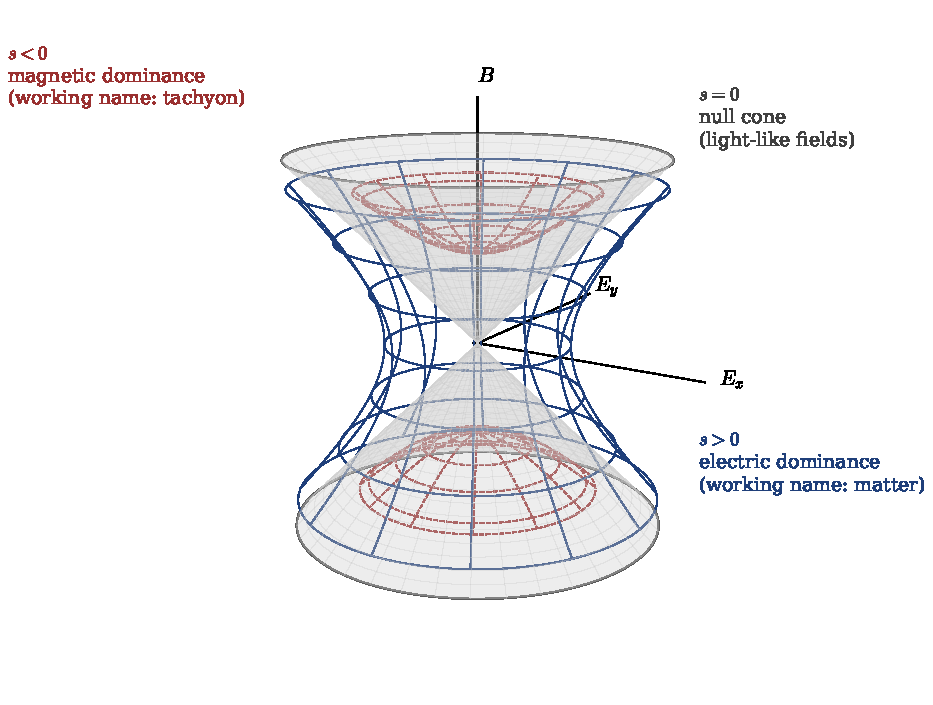
\includegraphics[width=0.78\textwidth]{figures/F2-sectors.pdf}
\caption{The three sectors of $s=z\cdot z$ on the slice where $\mathbf E\perp\mathbf B$, so that
$s=|\mathbf E|^2-|\mathbf B|^2$ is real ($\mathbf E$ horizontal, $\mathbf B$ vertical). Grey: the null cone
$s=0$ (light-like fields; the apex is the zero field). Solid: the level set $s=+1$ (electric dominance).
Dashed: the level set $s=-1$ (magnetic dominance). In the full space $\mathbb C^3$ the level sets
$s=c\neq0$ are the orbits of the Lorentz group $SO(3,\mathbb C)$, and the duality quarter turn
$z\mapsto iz$ maps the level $c$ to $-c$ (Proposition~\ref{prop:A-orbits}). The picture is a
three-dimensional slice of a six-dimensional space. \Established{} as geometry; the names matter and
tachyon are the working assignment of round v4.8.0-r07 and a \Reading.}
\label{fig:A-sectors}
\end{figure}


\subsection{What the compensator selects on a light field}
\label{sec:A-field-example}

The first test of a construction meant to describe light is a plane wave in vacuum: equal field
strengths and orthogonal fields. Take at one point $\mathbf E=a\mathbf e_x$, $\mathbf B=a\mathbf e_y$,
$a>0$, so $z=a(\mathbf e_x+i\mathbf e_y)$ and $s=0$. By \eqref{eq:A-Cz},
\begin{equation}
Cz=\frac a2(1+i)(\mathbf e_x+\mathbf e_y),\qquad Az=\frac a2(1-i)(\mathbf e_x-\mathbf e_y).
\label{eq:A-wave}
\end{equation}
The input has squared norm $|\mathbf E|^2+|\mathbf B|^2=2a^2$, each part has $a^2$; this is the
Pythagoras identity of the orthogonal splitting. The kept part has
$\mathbf E'=\mathbf B'=\tfrac a2(\mathbf e_x+\mathbf e_y)$, hence
$|\mathbf E'|^2=|\mathbf B'|^2=\mathbf E'\cdot\mathbf B'=a^2/2$ and
\begin{equation}
s(Cz)=2i\,|\mathbf E'|^2=i\,a^2\neq0 .
\label{eq:A-sC}
\end{equation}
The projection keeps the equality of the field strengths and destroys their orthogonality. The image
of a light-like field is not light-like.

This is general. For every field with $\mathbf E+\mathbf B\neq0$ the image $Cz$ has parallel electric
and magnetic parts, $\mathbf E'=\mathbf B'$. In the language of Section~\ref{sec:A-frames} it lies on
the rim $|b|=1$ of the state disk, the reference frame R, and never at the light-like centre P
(\rnd{r23}, Theoremlet r23.2) \Established. The kept and the removed part are each a selection; the
input is recovered only from both. A projection loses information, while symmetries do not
(\rnd{r16}, r16.6). The older reading of \texttt{prop:compensator}, in which $C$ produces the photon
from matter and its tachyon image, is therefore not supported: the quaternion identity $e_3=e_1e_2$
makes the \emph{product} $z\times J_Bz=2\,\mathbf E\times\mathbf B$ orthogonal to both inputs, not the
average (\rndold{r03}, r03.4). The Companion corrected the orthogonality clause of the proposition accordingly; its sentence
that $C$ produces the photon still stands in the main text and is superseded by \rnd{r23}.

\subsection{What the carrier does not give}
\label{sec:A-limits}

The carrier is a concrete algebra with checkable operations and invariants. It is not yet physics.
Four statements must be kept apart, and none implies the next: several data live on the same
mathematical carrier; several descriptions represent the same complete physical state; several states
belong to one theory and are connected by an active operation; different readouts of one state discard
different information. Proposition~\ref{prop:A-orbits} establishes the third for matter and tachyon
configurations; it says nothing about the second. The compensator is of the fourth kind.

In particular the carrier by itself identifies no particle. Which state is an electron and which a
photon requires the larger algebra
$\mathbb C\otimes\mathbb H\otimes\mathbb O$ and further named choices (Section~\ref{sec:B-particles}). The number of generations
is not derived there either; it is an input. It also contains
no dynamics: neither the evolution of $z$ nor an action that would fix a scale follows from the
algebra (Section~\ref{sec:act}). What it does fix is the frame structure of the next section.
